\section{Overview of Sensibility Testbed}\label{sec-overview}

In this section we discuss the steps required so that experiments 
can run on \sysname. 
%and the researcher's institution's \textit{local IRB}.
%
In the sections below, we present a high-level walkthrough of the steps 
required of the researcher and device owner, and 
introduce how the default policies are designed. 
%We further describe \sysname's design guideline 
%and the resulting testbed components. We also show the testbed operation.
We assume that Alice, a device owner, participates in 
the testbed, while a researcher, Rhonda, wants to runs code on \sysname 
using Alice's device, among other devices.

%\subsection{Walkthrough}\label{sec-walkthrough}

Alice decides to install Sensibility Testbed because she wants to 
altruistically help scientific progress.  She agrees to the privacy
policy for the platform and gives informed consent about the (Section~\ref{subsec:informed-consent})
type of research experiments she wants to participate in.  Alice also
may choose the granularity of data that her phone provides (Section~\ref{sec-alice-policy}), for 
example to block any possible access to her microphone.  At this point,
her smartphone is ready for researchers to use.  Alice may see experiments 
that are in the approval process, as
well as those that are running on her device, and choose
to opt-out at any time (Section~\ref{sec-alice-policy}). 

Now suppose that Rhonda, a researcher, wants to study the deployment of
different networking technologies in her city.  She wants to gather
the network type (3G, 4G, LTE, etc.), provider, and signal strength from
users all around the city.  Rhonda goes to the Sensibility Testbed website
and enters information about the sorts of data her experiment requires
into a form (Section~\ref{sec-ch}).  Rhonda decides that she can use randomized IDs in lieu 
of the smarthphone's cell ID, but requires the accurate carrier 
network information such as cellular signal strength and network type. 
%\cappos{please fill in / correct}
She also specifies that her experiment requires GPS data accurate to within
30m for her measurements and needs to update this every 10 seconds.
The Sensibility Testbed website takes her requirements and provides detailed
information for her IRB that Rhonda can use to describe Sensibility
Testbed and how the restrictions that Rhonda agreed to will be technically
enforced.

As is always the case with an IRB, Rhonda's IRB may at this point approve 
or ask her to revise the experiment and its requirements, providing any
changes to the Sensibility Testbed website.  Once approved, Rhonda submits 
the IRB approval to the Sensibility Testbed website.  If 
Rhonda's experiment requests access to sensors in a manner that is 
equal to or at a coarser level than a \emph{baseline} privacy (discussed in more detail
in Section~\ref{sec-policy-design}), her experiment will be immediately approved at this point.
If not, Rhonda's experiment is subject to an additional IRB check at NYU 
to ensure that her experiment will not violate Alice's consent or privacy and
that adequate controls can be put in place to replace the \emph{baseline}
privacy policies (Section~\ref{sec-repy}).

Now approved, Rhonda's experiment can be deployed on end user phones.  She
selects the devices she wishes to use on the Sensibility Testbed 
website, deploys her experiment, and collects the results (Section~\ref{sec-emt}).  
Even if Rhonda's rival Eve steals Rhonda's credentials and deploys a
malicious experiment, the experiment is blocked from accessing sensors except 
in the manner specified in the IRB policy.  Experiment code is blocked from 
reading the WiFi connection information (because this was not requested in
Rhonda's IRB) and is prevented from obtaining Alice's GPS information at a 
finer granularity or frequency than was listed. 
% \cappos{I resisted saying something about battery / malware
%here because these contributions are the focus of other papers.}
Alice is thus happy to let Rhonda perform her experiment, 
knowing that she is contributing to scientific progress without compromising 
her privacy. 
%
%\begin{figure}
%\center{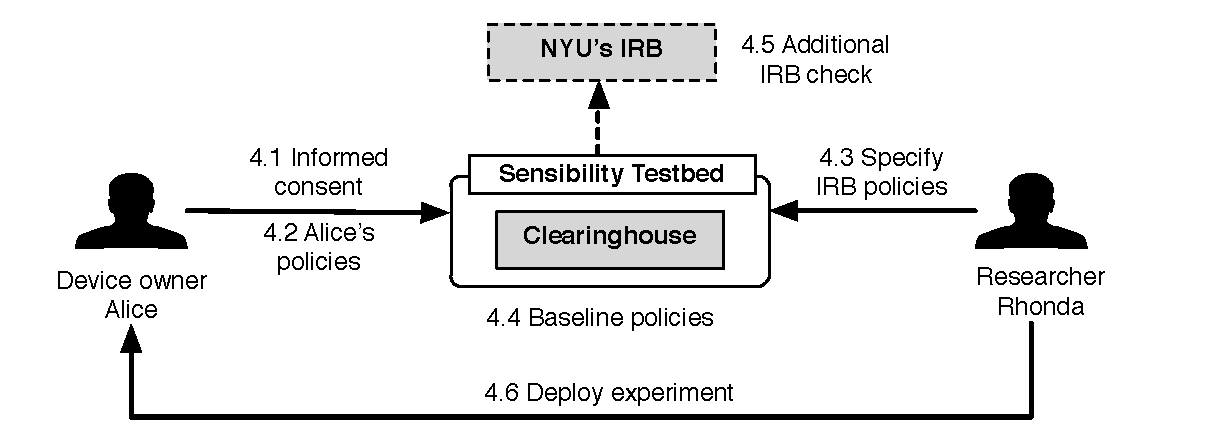
\includegraphics[width=\columnwidth, trim={.9cm .3cm 1.8cm .3cm}, clip]{figs/irb.pdf}}
%%\vspace*{-20pt}
%\caption{\small Overview of \sysname. \label{fig-walkthrough}}
%\end{figure}
%
%The above steps are shown in Figure~\ref{fig-walkthrough}, with each 
%step listed with the corresponding section number. 
This protocol for research with mobile device sensors has been approved by
the IRB at New York University (IRB \# 15-10751).  

\begin{comment}
%For Bob, the steps required to run an experiment include
%on \sysname roughly fall into two categories: 
%IRB approval for his experiment, and code deployment.
%Bob first %designs his experiment, and 
%possibly tests its feasibility on his own device (on which he can 
%use the same \sysname app but does not need IRB approval to access it). 
%Following this, he 
registers his experiment on the \sysname clearinghouse, where he 
specifies the sensors and sensor accuracy that his experiment 
requires through a web form. Suppose that the goal of Bob's experiment is to determine the cellular service
quality in major cities. His experiment therefore needs to obtain location information
of individual devices, their cellular service provider, network
type (3G, 4G, LTE, etc.), and signal strength. 
The clearinghouse's form provides Bob 
%summarizing the request. 
with a list of available sensors and their possible privacy configurations. 
Bob then requests approval for his experiment from his 
institution's IRB, supplying his experiment description using the clearinghouse form, the \sysname's approved 
IRB, and any additional information about the testbed as needed by his institution. 
The process how Bob specifies IRB policies is described in details in 
Section~\ref{sec-ch}. Once Bob's IRB approves the experiment, he 
uploads the confirmation to \sysname's clearinghouse, and is finally 
granted the permission to access devices to deploy his experiment 
and collect data, as will be described in Section~\ref{sec-emt}.

In order for Alice to participate in Sensibility Testbed,
she starts by installing the Sensibility Testbed app from 
the Android app store~\cite{sensibility-app}. After downloading the app, 
Alice is informed about the testbed's privacy and usage policy 
in a consent form and must give consent before participating.
She can opt out of the testbed by uninstalling the app, opt out of
an individual experiment, and set local sensor policies that
will supersede Bob's IRB policies (Section~\ref{sec-repy}). This
protocol for research with mobile device sensors has been approved by
the IRB at New York University (IRB \# 15-10751).  

Bob completes a series of steps to deploy his experiment on \sysname.
He first fills out a form at a \sysname website 
(Section~\ref{sec-ch}), which has a list of checkboxes for device sensors 
and text boxes indicating the precision and frequency that Bob can access 
each sensor. These boxes provide the default policies of \sysname, and 
Bob can only indicate data of coarser granularity. \jill{i thought this process was automated?}
Bob then downloads 
documents to provide to his IRB that 
explains the details about his experiment, \sysname and the technical 
restrictions his experiment will have. Bob then obtains IRB approval at 
his institution, provides his institution's IRB policies to the 
\sysname website, and signs up for his experiment. 

The form that Bob filled out on the \sysname website is used to
enforce a set of technical restrictions for his experiment.  This means
that even if Bob makes an error in his code or his code is malicious, his 
experiment is still restricted in the data it can acquire. 
\yanyan{how can restricting data prevent errors?} Therefore, Bob's IRB 
policies which request access to cellular signal strength and network type, would result 
in his experiment being blocked from reading the cellular roaming status and cell 
IDs. Note that the latter information is accessible with the same 
Android permission, but is blocked by \sysname.  This
protocol for research with mobile device sensors has been approved by
the IRB at New York University (IRB \# 15-10751).  

Note that the policies set limits to the precision of data that Bob can request
for many sensors (e.g., preventing access to the raw MAC address of the device).
If Bob has a legitimate need for this data and can appropriately secure it,
Bob can request such access by also passing his locally approved request 
through \sysname's IRB.  This additional check ensures not only that Bob's 
handling and access to the data is appropriate, but ensures that this does
not violate Alice's privacy and usage policy with the Sensibility Testbed.
%When Bob's IRB wants to access information that is more sensitive than
%what is described in NYU IRB, \yanyan{Justin, help!}  

Once Bob's experiment has been approved and the appropriate privacy
restrictions are identified, Bob can obtain remote devices, and run his experiment on the
devices of participants like Alice (Section~\ref{sec-emt}). On Alice's device, the app displays a 
list of running experiments and their policies. If Alice does not agree with
sharing her MAC address, she can opt out of Bob's experiment. 
%\cappos{how is this updated?  Does Alice see this before or after an 
%experiment may run?  How much "lead time" does Alice get to opt-out
%before the experiment happens?}
%\cappos{Do you want to say something about informed consent here or
%does it fit better later?} 
Alice's informed consent to Sensibility Testbed
ensures that Bob does not need to individually recruit Alice to include
her device in his study.

This work flow is shown in Figure~\ref{fig-walkthrough}. \jill{let's add how Bob gets the 
data from Alice's device in Figure 1} \sysname
acts as an intermediate between the device owner and researcher, 
where the device owners give their informed consent, and researchers
provide their IRB policies. The researchers do not recruit
device owners directly for each experiment, and the testbed infrastructure 
enforces the IRB policies on behalf of the researcher. 

\sysname's default policies are described next.
\end{comment}

%Device owners like Alice participate in Sensibility Testbed by p.

%These policies restrict what and how data can be accessed by the 
%researcher. 
%into data blurring layers that are enforced on
%mobile devices. Such a process can protect device
%owners' personal information. 
%Researchers' code runs in a sandbox that isolates the code from the 
%rest of the device host system. 
%To control the execution of code, Bob uses his own 
%desktop or laptop computer to manage the 
%experiments via the experiment manager. It deploys 
%and runs experiments in sandboxes on remote devices that are 
%acquired through the clearinghouse.

%\textbf{Usage scenario 1: Smartphone owner volunteers as a testbed participant.}
%Alice downloads the Sensibility Testbed app from the Google Play 
%Store~\cite{sensibility-app}, which will install Repy and other software on her phone.
%The app displays a consent form, \yanyan{cite link} containing the testbed's 
%general usage policy. Alice must review and must agree to this 
%policy before installation. If Alice gives her consent, her device will be 
%installed with the Repy sandbox, the native Android code to 
%start or stop the sandbox, and an interface to communicate with the testbed 
%infrastructure (particularly the clearinghouse, described below). 
%By agreeing to our general usage policy, any device 
%owner, regardless of age, country, or background, need only to opt into our testbed as a
%volunteer \textit{once}, at the time of app installation. 
%%As a result, an 
%%researcher like Bob who wants to conduct an experiment 
%%%requests devices through our clearinghouse, which assigns 
%%%them devices from a set of available resources. As a result, 
%%%the researcher
%%does not need to get consent from each subject for each individual
%%experiment. \lois{is the previous sentence needed? I don't think so} 
%The testbed thus greatly simplifies the process for both the 
%device owners and experimenters. 

